\RequirePackage[T1]{fontenc}
\documentclass[conference,10pt,letterpaper]{IEEEtran}
\usepackage{amsmath,amssymb,graphicx,booktabs,cite}
\usepackage{algorithm,algpseudocode}
\usepackage[hyphens]{url}
\usepackage[hidelinks]{hyperref}
\hypersetup{pdftitle={Exposing Cross-Group Parallelism in Layer-Aware Lookahead Construction for 3D FPGA Routing},pdfauthor={},pdfsubject={Anonymous expanded research manuscript},pdfkeywords={3D FPGA, parallel CAD, routing lookahead, semantics preservation}}
\newcommand{\speedup}{\ensuremath{\times}}
\newcommand{\Group}{\textsc{Group}}
\newcommand{\Pipe}{\textsc{Pipeline}}
\newcommand{\Flat}{\textsc{Flat}}
\newcommand{\Bound}{\textsc{Bounded}}
\newtheorem{proposition}{Proposition}
\newcommand{\PrimarySpeed}{$1.638\pm0.005$}
\newcommand{\PrimaryCache}{$1.000\pm0.009$}
\newcommand{\PrimaryBuild}{$7.144\pm0.266$}
\newcommand{\BnnScaling}{$12.006\pm0.167$}
\newcommand{\BnnGroupSixteen}{$3.123\pm0.033$}
\newcommand{\DlaScaling}{$12.253\pm0.296$}
\newcommand{\DlaGroupSixteen}{$3.123\pm0.001$}
\newcommand{\DlaFour}{$0.954\pm0.003$}
\newcommand{\BnnTwoDProcess}{$1.356\pm0.028$}
\newcommand{\BnnTwoDFlat}{$1.028\pm0.024$}
\newcommand{\BnnTwoDBuildFlat}{$1.002\pm0.044$}
\newcommand{\LargeThreeDProcess}{1.681}

\newcommand{\GemmRebuildMeanSD}{$1.638\pm0.005$}
\newcommand{\GemmReuseMeanSD}{$1.000\pm0.009$}
\newcommand{\ConfirmGemmMeanSD}{$1.091\pm0.008$}
\newcommand{\ConfirmSoftmaxMeanSD}{$1.121\pm0.030$}
\newcommand{\ConfirmReductionMeanSD}{$1.092\pm0.008$}

\makeatletter
\newcommand{\tableinput}[1]{\@@input #1 }
\makeatother
\title{Exposing Cross-Group Parallelism in Layer-Aware\\Lookahead Construction for 3D FPGA Routing}
\author{\IEEEauthorblockN{Anonymous Authors}}
\begin{document}
\maketitle
\begin{abstract}
Native multicore routing leaves costly lookahead construction insufficiently parallelized. We present a semantics-preserving decomposition for 3D FPGA lookahead: independent layer-aware floods, ordered cost reduction, and cross-group execution with reusable private workspaces. Slice-local interpolation and compact storage further expose scheduling and memory tradeoffs. On eight-core GEMM, construction falls from 149.56 to 20.95 seconds and process speedup is $1.638\pm0.005$\speedup. On two large 3D graphs, Pipeline scales approximately $12$\speedup\ from one to sixteen cores while group-local execution saturates. Native equivalence checks, full-routing experiments, and direct global-task controls establish the benefit of removing group barriers and a verified task boundary for future hardware acceleration.
\end{abstract}
\begin{IEEEkeywords}
3D FPGA, routing lookahead, multicore CAD, deterministic reduction, architecture exploration
\end{IEEEkeywords}

\section{Introduction}
Three-dimensional FPGA integration expands the architecture design space through stacked active fabrics, heterogeneous resources, and programmable vertical interconnects. Evaluating this space requires CAD tools that can both represent these structures and process their resource graphs efficiently. LaZagna demonstrates flexible architecture generation and evaluation, while Escaping Flatland improves placement through layer assignment, delay modeling, and 3D move operators~\cite{lazagna,flatland}. These advances increase the value of a fast routing backend: more candidate architectures and placements can be assessed within a fixed exploration budget. Changing connectivity or calibrated costs can require a new lookahead table even when the subsequent router already supports multiple CPU cores.

VPR's native parallel router does not make every part of a routing invocation parallel. The map-lookahead construction in our locked baseline enumerates representative wire samples and executes their graph searches sequentially. Increasing the routing worker budget therefore leaves a substantial initialization bottleneck. On a two-layer GEMM resource graph, stock VPR with eight physical cores spends $149.56\pm1.32$ seconds constructing lookahead, compared with $30.64\pm0.38$ seconds in routing, within a $331.05\pm1.36$-second process. Construction accounts for approximately 45\% of this process, including loading and checks. Optimizing only the routing search cannot remove that cost.

A direct first step is to execute the samples of each wire group concurrently. However, representative groups often contain only four samples. With a barrier after every group, assigning eight or sixteen workers still exposes at most four simultaneous sample searches. The challenge is to expose parallelism across groups while preserving the numerical model used by timing-driven routing. Equal-delay samples carry associated congestion costs; completion-order reduction can change the selected pair. In 3D, results additionally distinguish source and target layers, vertical wire directions, and missing slices. Naively parallelizing the surrounding loops can introduce write conflicts during interpolation.

We address these issues by separating native semantics from execution order. Each unchanged sample flood operates on private search state and produces a layer-indexed result. An ordered reduction preserves the native delay/congestion winner, while a global task stream removes group barriers. The implementation uses VPR's existing oneTBB worker budget. A bounded-token Pipeline overlaps searches and reductions; a direct global parallel loop provides an independent execution realization. We also analyze slice-local interpolation and compact intermediate storage to expose additional dependencies and resource tradeoffs.

Our contributions are the following.
\begin{enumerate}
\item \textbf{A semantics-preserving parallel decomposition.} We identify independent sample floods, retain source-relative coordinates and strict-delay tie semantics, and formulate ordered reduction as the correctness boundary between concurrent execution and the native map.
\item \textbf{Cross-group execution inside native VPR.} We replace group-limited concurrency with global sample scheduling, reusable private workspaces, and bounded in-flight results. Direct global-loop controls establish which improvements arise from removing group barriers, rather than attributing all gains to a particular library primitive.
\item \textbf{Explicit support for layer-aware construction and storage.} We preserve CHANZ sampling, all target-layer slices, native inter-layer cost semantics, and unsampled-layer completion. A slice dependency analysis permits equivalent commit schedules and reduces redundant interpolation scans; compact cells and a budgeted variant quantify the resulting storage/performance tradeoffs.
\item \textbf{Native validation from construction to routing workflows.} We evaluate 603 formal measurements across 2D and two-layer 3D inputs, separating 414 legal full-flow runs from 189 construction-only runs. Scaling, same-executable controls, cache sequences, memory diagnostics, and independent route checks connect the algorithmic decomposition to its practical benefit and remaining costs.
\end{enumerate}

Pipeline achieves \PrimarySpeed\speedup\ paired process speedup on eight-core GEMM. On BNN and DLA 3D graphs, its one-to-sixteen-core construction speedups are \BnnScaling\speedup\ and \DlaScaling\speedup, respectively. These results establish effective use of parallelism beyond individual groups. They also expose a concrete acceleration boundary for future GPU or FPGA engines: independent searches may be replaced while retaining an ordered, testable map-construction interface.

\begin{figure*}[t]
\centering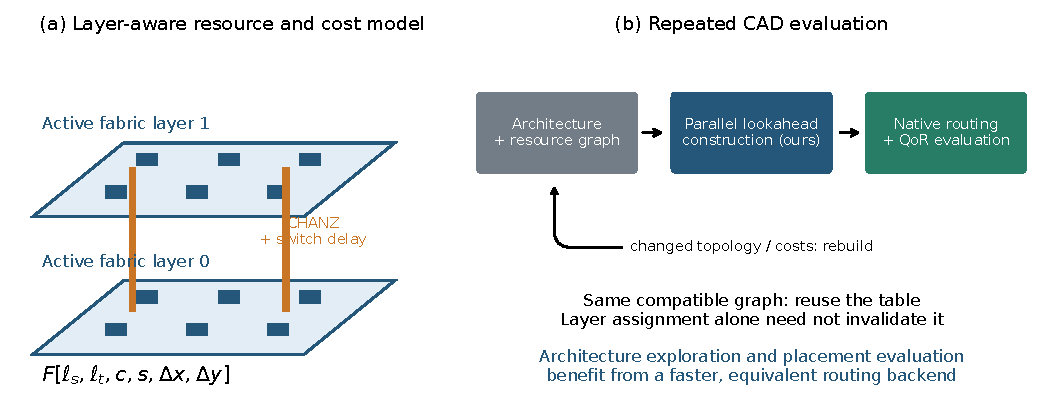
\includegraphics[width=.98\textwidth]{figures/expanded_context.pdf}
\caption{Research context. (a) Two active fabric layers connect through modeled vertical routing resources; the lookahead retains source/target layer identity. (b) Faster equivalent construction reduces the cost of evaluating changed resource graphs. Reusing a compatible graph permits caching; changing placement alone does not necessarily require reconstruction. The schematic is conceptual, not a physical implementation measurement.}
\label{fig:context}
\end{figure*}

\section{Background and Problem Formulation}
\subsection{3D Resource Graphs and Lookahead Semantics}
An FPGA routing-resource graph is a directed graph $\mathcal{R}=(V,E)$ whose vertices represent wires and pins, with capacity, location, type, and cost information. PathFinder-style negotiation resolves contention between routed nets~\cite{pathfinder}. VPR combines congestion and timing costs with an estimate of the remaining cost to a sink~\cite{vtr8,vtr9}. The sampled map-lookahead approach constructs these estimates by flooding representative wire starts and recording costs at relative destination coordinates~\cite{diversity}.

For a layered architecture, let the wire-cost table be
\begin{equation}
 F[\ell_s,\ell_t,c,s,\Delta x,\Delta y]=(d,q),
 \label{eq:map}
\end{equation}
where $\ell_s$ and $\ell_t$ are source and target layers, $c$ is channel type, $s$ is segment type, and $d,q$ are the retained delay and congestion estimates. A sampling group $g=(\ell_s,s,c)$ contains an ordered list of starts $R_g=(r_{g,0},\ldots,r_{g,n_g-1})$. Each sample can reach destinations on every layer. Missing entries are completed using native interpolation. Source/OPIN preprocessing and derived minima are additional parts of the full construction stage.

Our 3D inputs model two active fabric layers containing logic, DSP, and memory resources, connected by explicit vertical segments and inter-layer switches. The architecture specifies \texttt{axis=z} segments, upward/downward links, and fan-in-dependent switch delays. Actual routes contain CHANZ transitions between $(x,y,0)$ and $(x,y,1)$. Thus the 3D classification follows from architecture, connectivity, and routed paths together, rather than layer labels alone. We adopt the existing VTR multi-die model~\cite{third_dimension,multidie}; our contribution is its parallel construction, not the invention of vertical routing resources.

The native wire flood uses its existing indexed delay and congestion model. We preserve these computations, graph edges, sample choices, and traversal semantics. We do not replace the cost model with Manhattan distance or claim a new per-edge physical-delay model. In particular, the placement-delay refinement in Escaping Flatland~\cite{flatland} is a distinct contribution that motivates, but is not implemented by, this work.

\subsection{Available Threads Versus Available Work}
The stock executable already receives the same physical-core budget and enables native parallel routing in our process comparisons. Its wire-sampling loop remains sequential. Our within-group implementation, \Group, first exposes sample concurrency, but synchronizes before the next group. The cross-group implementations instead expose the union of all independent sample tasks.

Let $t_{g,j}$ denote ideal sample-search work, $W_g=\sum_jt_{g,j}$, and $W=\sum_gW_g$. Ignoring synchronization, memory contention, allocation, and reduction, lower bounds on search time under $P$ workers are
\begin{align}
 T_{\rm group}&\geq\sum_g\max\{W_g/P,\max_jt_{g,j}\},\\
 T_{\rm global}&\geq\max\{W/P,\max_{g,j}t_{g,j}\}.
 \label{eq:width}
\end{align}
The second schedule allows work from one group to occupy workers unavailable to the first. For ten groups of four equal-cost samples, group-local execution requires ten waves at both eight and sixteen cores. Global execution needs five and three waves, respectively. The sixteen-core discrete speedup limit of this example is $40/3=13.33$ relative to one core, rather than sixteen. This illustrates available task parallelism; it is not a measured CPU-utilization percentage or a guarantee of optimal scheduling.

\begin{figure*}[t]
\centering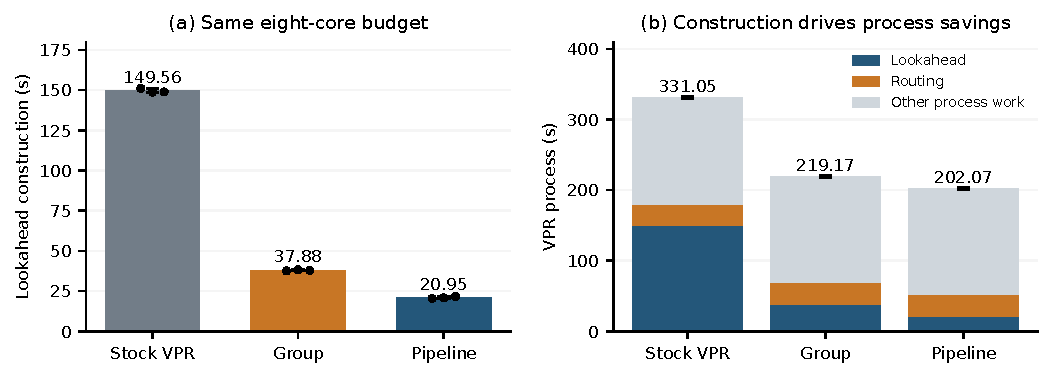
\includegraphics[width=.98\textwidth]{figures/expanded_motivation.pdf}
\caption{Measured GEMM motivation at the same eight-physical-core budget, three repeats per implementation. (a) Complete lookahead construction: Stock $149.56\pm1.32$ s, Group $37.88\pm0.37$ s, Pipeline $20.95\pm0.64$ s. (b) Full fixed-input VPR process; the residual includes loading, checking, and all other process work. Bars show means; error bars show sample SD. Stock already enables native parallel routing. Group is our within-group implementation, not an upstream baseline.}
\label{fig:motivation}
\end{figure*}

\subsection{Related Parallel and 3D CAD Methods}
MultiQueue routing exposes parallelism within an individual connection search using relaxed priority ordering~\cite{multiqueue}. Our unit of concurrency is an unchanged flood: we parallelize independent samples and groups while maintaining each flood's native search order. The two granularities can potentially be combined, but that composition requires separate validation.

VPR offers alternative routing algorithms, compressed lookahead, and table read/write support~\cite{vproptions}. Compressed lookahead trades representation and sampling choices against construction cost; our main comparisons preserve the original map. The locked compressed implementation accepts only a single layer, so its rejection of a two-layer input is treated as an applicability limitation. Compatible 2D alternatives are evaluated separately. Global \texttt{parallel\_for}, private workspaces, and ordered pipelines are existing oneTBB mechanisms~\cite{tbb}; the contribution is the dependency decomposition and equivalent native integration that make those mechanisms useful for layer-aware construction.

LaZagna expands the range of realizable 3D architectures, including vertical connection patterns and heterogeneous layers~\cite{lazagna}. Escaping Flatland improves the quality of placements on such architectures~\cite{flatland}. Our work complements these objectives by reducing the cost of constructing an unchanged routing heuristic. A faster backend can support more architecture candidates and repeated placement evaluation without confounding algorithmic quality with a changed heuristic.

\section{Semantics-Preserving Cross-Group Construction}
\subsection{Independent Floods With Private State}
For each native group $g$, sample selection follows the original reference locations, segment and direction filters, and fallback search for unusual wire types. We retain groups for supported X, Y, and Z channel types and respect layers without inter-cluster programmable resources. A task descriptor identifies its group, sample index, and start RR node. Its output $C_{g,j}[\ell_t,\Delta x,\Delta y]$ includes every destination layer.

Every worker owns an expanded bitmap, visited-cost array, priority queue, and sample output. The resource graph and cost data are read-only during construction. A worker may reuse its allocated workspace for subsequent tasks, but resets search state for every new flood. Reuse of storage therefore does not merge searches or propagate labels from a different source. The original full-device bounding box spans all layers, so paths can traverse native CHANZ resources while retaining layer-dependent costs.

Source identity must survive the decomposition. Consider two starts at $x=0$ and $x=5$ reaching a pin at $x=6$ with delays 1 and 2. The native samples contribute to displacement buckets 6 and 1, respectively. A nearest-source search keeping only the cheaper label at the pin loses the second contribution. Consequently, shared destinations do not justify replacing the samples with a single unlabeled multi-source flood. Even repeated start RR IDs require matching recording context and search constraints before exact reuse is valid. We retain all selected samples.

\subsection{Ordered Reduction and Correctness}
The native smallest-entry rule replaces a populated cell only when the new delay is strictly smaller. Its congestion value must remain paired with that delay. For finite valid values, the winner at a cell $u$ is
\begin{equation}
 j^*(u)=\arg\min_{j:C_{g,j}(u)\text{ occupied}}(d_{g,j}(u),j).
 \label{eq:ordered}
\end{equation}
The cell contains $(d_{g,j^*},q_{g,j^*})$, not two independently minimized scalars. We implement the native insertion and occupancy predicates directly, rather than relying on a generic floating-point tuple minimum.

\begin{proposition}
Assume native sample selection and within-flood visitation are unchanged, recorded valid delays are finite, and final commits and interpolation follow the native order. Private sample execution followed by original-order strict-delay reduction yields the same wire-cost table as serial sample execution.
\end{proposition}
\noindent\emph{Proof.}
At each cell, one sample's representative is the minimum-delay entry first encountered within that sample. Native serial execution concatenates these per-sample visitation sequences. Reducing their representatives in sample order selects the minimum delay in the concatenation and retains its earliest associated congestion on ties. Thus each populated cell agrees; missing cells retain the same occupancy state. Identical commits and interpolation then produce identical final cells. The argument is independent of task completion order. $\square$

This proposition does not license arbitrary reassociation of exceptional floating-point values. NaNs, invalid sentinels, signed zeros, and occupied-but-invalid states are handled by the native insertion rules and separate representation tests. It also does not require final parallel route files to be byte-identical: routing has its own concurrent state and trajectory.

\begin{algorithm}[t]
\caption{Layer-aware cross-group Pipeline construction}
\label{alg:pipeline}
\footnotesize
\begin{algorithmic}[1]
\Require RR graph $\mathcal R$, native cost data, worker budget $P$
\Ensure Native-equivalent wire table $F$
\State $\mathcal G\gets$ native ordered $(\ell_s,s,c)$ groups
\State $J\gets[\ ]$; initialize native-empty group tables $B_g$
\For{$g\in\mathcal G$ in native order}
 \State $R_g\gets\Call{NativeSelect}{\mathcal R,g}$
 \For{$j=0,\ldots,|R_g|-1$}
  \State append $(g,j,R_g[j])$ to $J$
 \EndFor
\EndFor
\State $Q\gets\min(|J|,2P)$ in-flight sample tokens
\Statex \textit{Ordered producer:}
\State Emit descriptors from $J$ in order, subject to $Q$
\Statex \textit{Parallel worker for descriptor $(g,j,r)$:}
\State $W_t\gets$ private reusable workspace; reset its labels/queue
\State $C\gets\Call{NativeFlood}{\mathcal R,r,W_t}$
\State Publish $(g,j,C)$ with all target-layer cells
\Statex \textit{Ordered consumer, in descriptor order:}
\State $B_g\gets\Call{NativeStrictMerge}{B_g,C}$
\State Release $C$ and its token
\Statex \textit{After pipeline completion:}
\For{$g\in\mathcal G$ in native order}
 \State $F\gets\Call{NativeCommitAndInterpolate}{F,g,B_g}$
\EndFor
\State Run unchanged source/OPIN and derived-minimum construction
\end{algorithmic}
\end{algorithm}

\subsection{Three Execution Schedules}
\textbf{Group-local execution.} \Group\ allocates private sample results for one group, executes its floods in parallel, and reduces them in original order. The next group starts after this barrier. This establishes sample independence but limits active work to the current group's sample count.

\textbf{Direct global execution.} \Flat\ materializes the same ordered descriptors for all groups, executes them with one global \texttt{parallel\_for}, then reduces all results in descriptor order after the join. Workspace allocation is thread-local and spans groups. This schedule isolates the effect of globally exposing the task set without an ordered pipeline.

\textbf{Ordered pipeline execution.} Algorithm~\ref{alg:pipeline} uses an ordered producer, parallel flood body, and ordered consumer. At most $\min(S,2P)$ sample results are in flight for $S$ total samples. Later groups can execute while an earlier group is still outstanding. Results are reduced and released incrementally; commits retain native group order. Head-of-line waiting at the consumer and per-flood imbalance can still limit speed. \Flat\ and \Pipe\ share task enumeration, flood code, result representation, and native commit order in their direct comparison.

The global implementations also change allocation lifetimes and search/reduction overlap. We therefore interpret Flat-to-Pipeline measurements as a comparison of complete execution realizations, not a measurement of scheduling overhead alone. The TBB budget limits allowed parallelism, while observed workspace count is measured separately; it is not assumed to equal the thread budget in every run.

\begin{figure*}[t]
\centering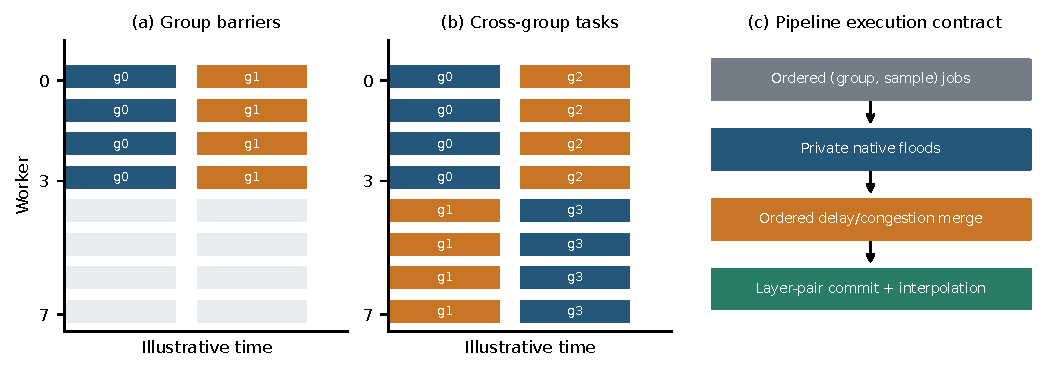
\includegraphics[width=.98\textwidth]{figures/expanded_schedule.pdf}
\caption{From local concurrency to global task parallelism. The equal-length schedule is illustrative: a four-sample group cannot occupy eight workers, whereas samples from successive groups can. The actual implementation preserves the ordered map-reduction boundary while allowing independent floods to complete out of order.}
\label{fig:schedule}
\end{figure*}

\subsection{What the Algorithm Preserves for 3D FPGA Routing}
The layer dimension affects the algorithm at several specific points.
\begin{enumerate}
\item \textbf{Layer- and direction-aware task enumeration.} The task key retains source layer, segment, and channel type, including CHANZ. Native vertical direction selection and fallback behavior are preserved. These are inherited graph semantics explicitly maintained by the parallel implementation.
\item \textbf{Cross-layer search and destination recording.} Each flood uses the complete multilayer graph. Its result is indexed by target layer as well as displacement, so equal $(\Delta x,\Delta y)$ on different layers cannot alias. Layer crossing is represented by native resources and costs, not an assumed constant geometric penalty.
\item \textbf{Layer-pair-specific reduction and completion.} Private results merge only into the matching source-layer group, retaining all target layers. Interpolation operates within fixed layer-pair slices, with native completion for unsampled or disabled source layers.
\item \textbf{Resource scaling with layers.} Private maps contain $LWH$ cells and the final map contains layer-pair slices. Token limits and the optional compact representation make this cost explicit instead of silently replicating the entire global map per worker.
\end{enumerate}
The current native CHANZ selection path includes assumptions specific to the tested one-/two-layer configurations. Synthetic higher-layer interpolation tests do not establish a native arbitrary-layer implementation. The algorithmic treatment is layer-aware, but performance portability to other layer counts and vertical fabrics remains a separate evaluation.

\section{Slice Dependencies and Resource-Aware Variants}
\subsection{Equivalent Slice Completion}
An interpolation call may traverse multiple layers without creating a numerical dependence between them. Inspection of both native neighbor helpers shows that $(\ell_s,\ell_t,c,s)$ stays fixed: only $(\Delta x,\Delta y)$ varies. Thus distinct layer-pair slices are independent, while entries within a slice can depend on earlier filled entries. The original outer-$x$, inner-$y$ scan and floating-point accumulation order must remain unchanged.

The commit for a group overwrites its complete source-layer region, including initially invalid entries. Earlier provisional interpolation in that region is therefore superseded. Once a completed slice is filled, subsequent native calls retain valid entries. Under unique group keys, full-region commits, and no partial-map consumer, these properties permit two equivalent schedules: defer interpolation until all raw groups have been committed, then fill each used channel/segment combination once; or commit and fill only each completed group's source-layer slices, followed by defaults for unsampled layers. Algorithm~\ref{alg:slices} gives the latter.

\begin{algorithm}[t]
\caption{Equivalent source-layer slice completion}
\label{alg:slices}
\footnotesize
\begin{algorithmic}[1]
\Require Completed group table $B_g$, $g=(\ell_s,s,c)$
\State Commit every raw cell of $B_g$ to $F[\ell_s,:,c,s,:,:]$
\For{every target layer $\ell_t$}
 \State $U\gets F[\ell_s,\ell_t,c,s,:,:]$
 \For{$x$ in native outer-loop order}
  \For{$y$ in native inner-loop order}
   \If{$U[x,y]$ requires completion}
    \State Apply native neighbor rule in native summation order
   \EndIf
  \EndFor
 \EndFor
\EndFor
\State Publish group completion; release its intermediates
\Statex \textit{After all sampled groups complete:}
\For{each used $(s,c)$ and unsampled source layer $\ell_s$}
 \State Apply the same native slice completion for every $\ell_t$
\EndFor
\State Leave entirely unused $(s,c)$ combinations untouched
\end{algorithmic}
\end{algorithm}

Let $L$ be the number of layers, $K$ the used channel/segment combinations, and $A=WH$. If every layer supplies every group, repeated whole-table traversal performs $KL^3A$ missing-cell checks. Completing each final slice once requires $KL^2A$. This reduces redundant interpolation scans; it does not reduce the number of floods or imply an $L$-fold overall speedup. Its additional value is enabling early release of completed groups.

\subsection{Compact Cells and Bounded Active Results}
In native smallest-entry mode, an intermediate cell needs one occupied flag and the retained $(d,q)$ pair. We implement a scalar cell preserving the vector-based insertion semantics, including the distinction between occupancy and numerical validity. On the measured ABI, a vector header occupies 24 bytes before any element allocation, while the scalar cell occupies 12 bytes. This reduction concerns the intermediate representation, not the entire process RSS.

The \Bound\ variant allocates a bounded set of private sample tables and search workspaces. When a group's final sample completes, its worker performs the original-order reduction into the first table, commits and fills that group's slices, and releases the remaining tables. An acquire/release completion counter publishes preceding writes. The implementation uses bounded batches with barriers; a group exceeding the table budget falls back to serial insertion into one table. Slice-only, compact-cell, and bounded variants are evaluated separately from the primary Pipeline.

For $M=LWH$, $G$ allocated group tables, and $S$ total samples, the table-count relationships are summarized in Table~\ref{tab:storage}. Group metadata and task descriptors add $O(G+S)$ storage. Search labels, priority queues, allocator state, the resource graph, and the final map are additional. A workspace estimate cannot provide a hard RSS limit because queues and allocator caches can grow.

\begin{table}[t]
\centering\footnotesize
\caption{Intermediate-table structure. Counts exclude the common final map and resource graph; vector payloads and search workspaces are additional. $S_g$ is the current group's sample count; $K_a$ is the bounded active-slot count.}
\label{tab:storage}
\setlength{\tabcolsep}{3pt}
\begin{tabular}{lrrl}
\toprule
Method & Sample tables & Group tables & Cell backing \\
\midrule
Group & $S_g$ & 1 & $24M(S_g+1)$ \\
Flat & $S$ & $G$ & $24M(S+G)$ \\
Pipeline & $\min(S,2P)$ & $G$ & $24M[G+\min(S,2P)]$ \\
Bounded & $K_a$ & in-place & $12MK_a$ \\
\bottomrule
\end{tabular}
\end{table}

\subsection{Native Integration and Layered Validation}
The implementation operates inside native VPR rather than replacing its router with a graph-only proxy. Two bounding-box notification repairs are shared by the CPU variants; these maintain parallel-router state but can change routing trajectories relative to Stock. We therefore distinguish Stock comparisons from same-repair, same-executable method comparisons. The repairs are integration prerequisites, not claimed first discoveries of those upstream issues.

Validation has complementary layers. Ordered-reduction enumeration covers 21,825 permutations. Extracted native interpolation tests cover 2,400 sparse fixtures over 1, 2, 3, 4, and 8 layers, including unsampled slices; two equivalent reorderings yield 4,800 bitwise comparisons with zero differences. Mutations that exchange the $x/y$ scan or omit unsampled-layer completion fail 1,905 and 1,902 fixtures, respectively. Scalar-cell tests cover 100,000 fixtures and 1,551,076 bitwise field comparisons, including exceptional values. Finally, native runs compare serialized wire maps and, for complete routes, apply native FULL checking and independent original-VPR FULL/STA verification. Wire-map equality does not assert equality of every derived source/OPIN structure or final route trajectory.

\section{Experimental Methodology}
\subsection{Input Workloads and 3D Classification}
Table~\ref{tab:datasets} lists the inputs used in the main performance studies. They combine neural-network compute circuits, DSP/arithmetic designs, and traditional logic benchmarks. A case consists of architecture XML, BLIF, a packed netlist, fixed placement, and frozen RR graph. Input matrices or neural-network training samples are not supplied to the router; these are hardware netlists mapped onto the listed fabrics.

The KOIOS-derived 3D model and Hecate 3D model contain two active layers and explicit CHANZ resources. The native k6 architecture and original KOIOS 2D architecture are single-layer controls without CHANZ nodes. BNN appears on both a 3D and a separately prepared 2D fabric; this tests applicability, not a matched physical-quality comparison between 2D and 3D. Different placement seeds on a fixed architecture can share a resource graph and are not counted as independent graph topologies.

\begin{table*}[t]
\centering\scriptsize
\caption{Dataset inventory. Grid dimensions are $X\times Y\times L$; $L=2$ rows are 3D, $L=1$ rows are 2D. Nodes and edges are in millions; CHANZ counts are exact. Nets exclude global/unrouted-empty nets. Blocks are placed clustered blocks. Width is 100 for the first seven rows and native k6 cases, 120 for BNN-3D/LSTM/DLA and BNN-2D. The latter 3D graph counts are taken from the actual width-120 XML. Two layouts of a circuit share the reported size.}
\label{tab:datasets}
\setlength{\tabcolsep}{3pt}
\begin{tabular}{lllrrrrrrr}
\toprule
Circuit & Workload type & Fabric & Grid & Layouts & Blocks & Nets & Nodes (M) & Edges (M) & CHANZ \\
\midrule
\tableinput{tables/expanded_datasets.tex}
\bottomrule
\end{tabular}
\end{table*}

\subsection{Cohorts and Experimental Boundaries}
The evidence comprises 603 formal records: 414 legal full-flow runs and 189 construction-only measurements. Table~\ref{tab:cohorts} separates the cohorts so neither repeated controls nor successful subsets inflate the workload count. The original 222 full-flow records contain GEMM timing/scaling, fresh-layout studies, three-circuit confirmation, and storage ablation. New complete-flow cohorts add a three-layout 3D subset, four k6 layouts, clma, and BNN-2D. Separate construction-only cohorts include all three large 3D graphs, regardless of their route outcome.

The three-layout width-120 full-flow subset was selected by a declared baseline qualification: LSTM seed 2 and both BNN seeds. The original six-layout set retains three successes and three failures; DLA seeds 1/2 and LSTM seed 1 are not silently replaced. All three graphs remain in the graph-only construction study. Construction experiments stop native routing after one iteration; their valid construction timers and maps do not establish legal complete routes. Pilots, 36 new full-flow qualification runs, 18 instrumented diagnostics, six compressed-map alternatives, and 90 cache-batch processes are reported outside the 603 formal records.

\begin{table*}[t]
\centering\footnotesize
\caption{Formal evidence cohorts. Runtime repeats are within fixed configurations, normally $n=3$; fresh layouts have one timing observation per configuration. Host labels distinguish execution cohorts, not resource exclusivity.}
\label{tab:cohorts}
\setlength{\tabcolsep}{4pt}
\begin{tabular}{llrlp{7.0cm}}
\toprule
Cohort & Scope & Runs & Host & Design and purpose \\
\midrule
Original three-way/extension & Full flow & 66 & A & GEMM: three variants and 4/8/16-core extension; alu4/diffeq/s38417: two fresh layouts each. \\
Independent confirmation & Full flow & 36 & A & GEMM, softmax, reduction; Group/Pipeline; rebuild/cache. \\
Representation ablation & Full flow & 120 & A & GEMM/elliptic; five implementations; 4/8 cores; rebuild/cache. \\
Large 3D construction & Construction & 36 & A & BNN/LSTM/DLA; Stock, fixed-serial, Group, Pipeline; eight cores. \\
Qualified large 3D subset & Full flow & 72 & A & Three layouts, two circuits; four arms; rebuild/cache; eight cores. \\
Independent k6 architecture & Full flow & 96 & A & tseng/des, two layouts each; four arms; rebuild/cache. \\
Core scaling & Construction & 90 & B & BNN/DLA/tseng; Group/Pipeline; 1/2/4/8/16 cores. \\
Direct global-loop controls & Construction & 54 & C & BNN/DLA/clma; Group/Flat/Pipeline; 8/16 cores. \\
clma complete routing & Full flow & 12 & C & One layout; Stock/Group/Flat/Pipeline; eight cores. \\
Original KOIOS 2D BNN & Both & 21 & C & Twelve full-flow and nine construction runs; eight cores. \\
\bottomrule
\end{tabular}
\end{table*}

\subsection{Baselines, Platform, and Timing}
The baseline is VTR commit \texttt{0b912334fdd8}, with GNU C++ 11.4 release builds and assertion level 2. Stock uses the original executable. Fixed-serial retains the same CPU-variant state repairs with sample parallelism disabled; Group enables per-group sample parallelism; Flat and Pipeline expose all groups. All full-flow arms use native parallel routing, the same worker budget, the same fixed inputs, and comparable map-output settings. Flat here denotes globally flattened \emph{lookahead tasks}, not VPR's separate flat-routing mode, which is disabled.

Measurements use Intel Xeon Gold 6530 CPU instances with one logical CPU per selected physical core and affinity within one NUMA node. Original/width-120/k6 measurements use the original instance; scaling and flat-control cohorts use additional shared instances. We retain the actual command, environment, topology, affinity, executable hash, and input hashes. Cohorts on different instances are never paired or pooled. Physical-core exclusivity is not established.

Construction time $T_{\rm LA}$ is the complete native lookahead timer: wire sampling, interpolation, source/OPIN work, and derived minima, excluding RR loading and map serialization. Process time $T_{\rm proc}$ includes fixed-input loading, lookahead, routing, native checking/STA, and uniform map output. Workflow time additionally includes independent original-VPR readback/checking. These process measurements do not execute new synthesis, packing, placement, or RR generation. Performance runs disable diagnostic counters. A shared-cache comparison uses the same qualified wire map; native source/OPIN work may still execute.

\subsection{Statistics, Quality, and Audit}
For each fixed configuration, times and paired ratios are reported as arithmetic mean $\pm$ sample SD. For repeat $r$,
\begin{equation}
 s_r=\frac{T_{{\rm control},r}}{T_{{\rm candidate},r}},\quad
 \bar{s}=\frac{1}{n}\sum_rs_r,\quad
 \sigma_s=\sqrt{\frac{\sum_r(s_r-\bar{s})^2}{n-1}}.
\end{equation}
We compute ratios before averaging; dividing mean times is a different statistic. SD describes the observed repetition variability and is not a confidence interval. Single-observation configurations have no estimated SD. Figures show mean/SD and, where space permits, individual observations. All raw measurements are retained in the artifact.

Cross-circuit summaries first take the geometric mean of per-layout mean paired ratios within each circuit, then the geometric mean across circuits. This gives equal circuit weights; BNN's two layouts do not receive twice LSTM's weight. Separate cache modes, timing scopes, and host cohorts are not combined. This manuscript consistently recomputes mean/SD summaries from frozen observations; original experimental protocols and selection records are retained unchanged.

Full-flow acceptance requires zero overuse, native and independent FULL/STA checks, preserved route identity through independent readback, and CPD and wirelength each within $+5\%$ of the paired control. Map-equivalent comparisons additionally require the reference wire-map bytes. Construction-only validity requires a complete positive build timer before routing, reference-map equality, and the prescribed capped exit. Failed qualifications are retained in their attempted denominators. These distinctions prevent construction success from being interpreted as routing success.

\section{Results}
\subsection{From Native Parallel Routing to Parallel Construction}
Figure~\ref{fig:motivation} shows the distinction between requesting multiple routing workers and exposing construction work. On the same eight-core GEMM input, mean construction time falls from 149.56 s in Stock to 37.88 s in Group and 20.95 s in Pipeline. The paired Stock-to-Pipeline construction speedup is \PrimaryBuild\speedup, and its process speedup is \PrimarySpeed\speedup. This is an observed bottleneck in the locked native flow, not a claim that every VPR routing algorithm has poor scaling on every design.

The construction-only study repeats the comparison across all three large 3D graphs (Table~\ref{tab:component}), including those whose full routes fail qualification. Same-executable fixed-serial controls distinguish the sample-parallel contribution from the integration repairs. Group reduces construction substantially; Pipeline further improves it by approximately $1.9$--$2.0$\speedup\ at eight cores. Serial and Group results demonstrate why the cross-group step matters beyond simply enabling a parallel option.

\begin{table*}[t]
\centering\footnotesize
\caption{Complete lookahead construction on all three width-120 3D graphs at eight physical cores. Times are seconds; entries are mean $\pm$ sample SD ($n=3$). Ratio columns are paired construction speedups. The one-iteration route tails are not counted as legal full routes.}
\label{tab:component}
\setlength{\tabcolsep}{5pt}
\begin{tabular}{lrrrrrr}
\toprule
Graph & Stock & Fixed-serial & Group & Pipeline & Stock/Pipeline & Group/Pipeline \\
\midrule
\tableinput{tables/expanded_component.tex}
\bottomrule
\end{tabular}
\end{table*}

\subsection{Scaling Beyond the Group Width}
Figure~\ref{fig:scaling} reports a separate 1/2/4/8/16-core construction cohort on three graphs. BNN and DLA have ten nonempty groups with four samples each. Their Group construction time saturates after four cores, while Pipeline continues improving through sixteen. Relative to its own one-core implementation, Pipeline obtains \BnnScaling\speedup\ on BNN and \DlaScaling\speedup\ on DLA. At sixteen cores, its gains over Group are \BnnGroupSixteen\speedup\ and \DlaGroupSixteen\speedup. This directly supports removing the group-local parallel-width limit.

The benefit depends on task availability and cost. The tseng 2D input has only eight samples, so sixteen workers cannot expose sixteen independent floods. Its subsecond stage is also sensitive to timer granularity. DLA's four-core Group-to-Pipeline ratio is \DlaFour\speedup, showing that cross-group overhead can outweigh its benefit when a group already supplies enough work. Approximately twelvefold sixteen-core scaling therefore establishes substantial additional concurrency, not perfect utilization or a universal speedup guarantee.

\begin{figure*}[t]
\centering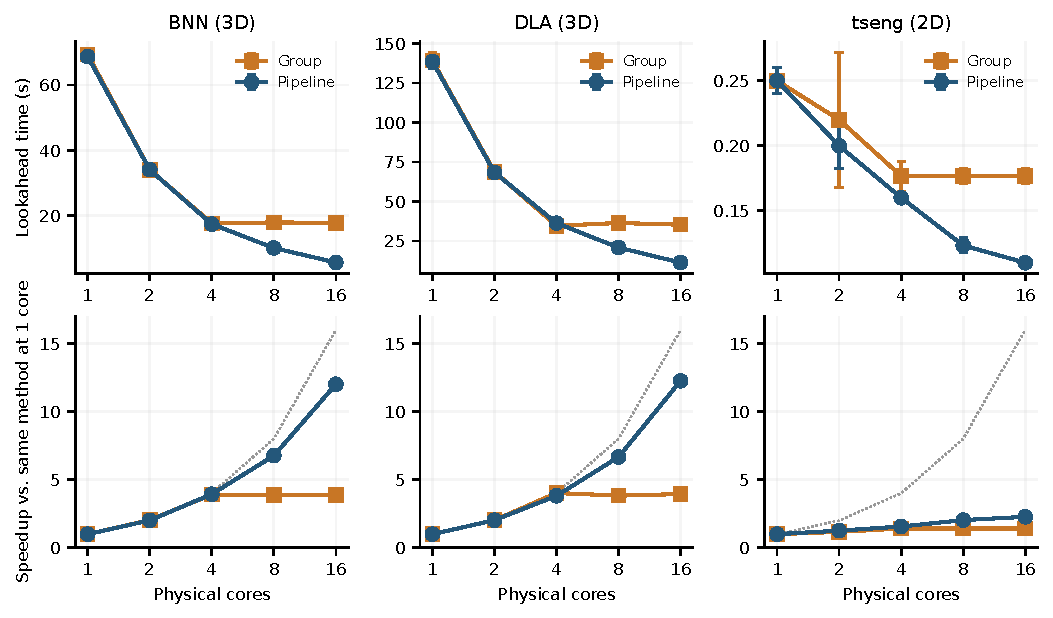
\includegraphics[width=.98\textwidth]{figures/expanded_scaling.pdf}
\caption{Construction scaling on host B, with three repeats at each core count. Top: mean construction wall time and sample SD. Bottom: paired speedup relative to the same method at one core; the dotted line is ideal linear scaling. Group saturates near the four-sample group width on BNN/DLA, while Pipeline exposes forty samples globally. tseng has only eight tasks. No process speedup or legal-route claim is derived from this capped-routing cohort.}
\label{fig:scaling}
\end{figure*}

\subsection{Direct Global-Loop Controls}
Table~\ref{tab:flat} compares Group, Flat, and Pipeline using one executable and the same task-generation/flood code. Both global implementations substantially outperform Group on large 3D graphs at eight and sixteen cores. Their mutual differences are much smaller: the BNN/DLA Flat-to-Pipeline mean ratios range from 0.995 to 1.029. Thus the dominant result is the benefit of exposing all independent groups. Pipeline's incremental release and bounded in-flight sample tables provide a distinct implementation tradeoff, but the current evidence does not establish that it is universally faster than direct global execution.

The larger 2D BNN also benefits: Group construction takes $7.75\pm0.27$ s, compared with $4.23\pm0.13$ s for Flat and $4.16\pm0.10$ s for Pipeline. The tiny clma stage has greater relative variability; retaining all observations prevents an apparently large ratio from being interpreted as a stable scheduling effect.

\begin{table*}[t]
\centering\footnotesize
\caption{Direct global-task controls on host C. Entries are mean $\pm$ sample SD ($n=3$); times are complete construction seconds, ratios are paired stage speedups. Flat is global \texttt{parallel\_for} with original-order reduction. BNN and DLA rows without a 2D suffix are 3D.}
\label{tab:flat}
\setlength{\tabcolsep}{5pt}
\begin{tabular}{lrrrrrr}
\toprule
Graph & Cores & Group & Flat & Pipeline & Group/Flat & Flat/Pipeline \\
\midrule
\tableinput{tables/expanded_flat.tex}
\bottomrule
\end{tabular}
\end{table*}

\subsection{Legal Full-Flow Benefit and Quality}
Table~\ref{tab:full} combines absolute process times and paired speedups, retaining the cohort and cache distinction. On the declared 3D conditional subset, Stock-to-Pipeline mean ratios are 1.638, 1.702, and 1.747 for LSTM seed 2 and BNN seeds 1/2. The equal-circuit geometric aggregate is \LargeThreeDProcess\speedup; the Group-to-Pipeline aggregate is 1.090\speedup. All nine rebuild pairs improve over both Stock and Group. The original three failed layouts remain outside this conditional full-flow claim and inside the broader construction evaluation.

\begin{table*}[t]
\centering\scriptsize
\caption{Legal full-process results at eight physical cores, mean $\pm$ sample SD ($n=3$). B: rebuild; C: common cache. Times are seconds; final columns are paired process speedups. GEMM and the large-3D/k6 rows are separate host-A cohorts; clma/BNN-2D are host C. Fixed-S is the repaired serial-construction control. ``--'' denotes an arm not present in that cohort. Preparation and independent-check time are excluded from these process times.}
\label{tab:full}
\setlength{\tabcolsep}{2.5pt}
\begin{tabular}{llrrrrrrr}
\toprule
Case & Mode & Stock & Fixed-S & Group & Pipeline & Flat & Stock/Pipeline & Group/Pipeline \\
\midrule
\tableinput{tables/expanded_full.tex}
\bottomrule
\end{tabular}
\end{table*}

For the 72 formal conditional-subset runs, all native and independent legality checks pass. Pipeline's largest CPD increase relative to Stock is 0\%, with maximum wirelength increase about 0.091\%. Relative to Group, the largest CPD and wirelength increases are about 0.165\% and 0.041\%. These changes satisfy the quality gate while showing that equal wire maps do not force identical parallel routing trajectories. Stock includes the state-repair difference; the same-repair controls and phase/cache measurements provide more specific attribution.

The original independent confirmation also retains nine improving rebuild pairs on GEMM, softmax, and reduction. Group-to-Pipeline process speedups are \ConfirmGemmMeanSD\speedup, \ConfirmSoftmaxMeanSD\speedup, and \ConfirmReductionMeanSD\speedup. The new k6 architecture yields an equal-circuit Stock-to-Pipeline rebuild aggregate of 1.129\speedup; individual small-design timings have greater relative uncertainty. On the original KOIOS 2D BNN, the full-process Stock-to-Pipeline result is \BnnTwoDProcess\speedup. Its Flat-to-Pipeline process ratio is \BnnTwoDFlat\speedup, whereas the construction ratio within those same full runs is \BnnTwoDBuildFlat\speedup. A small process difference therefore cannot automatically be assigned entirely to construction scheduling.

\begin{figure*}[t]
\centering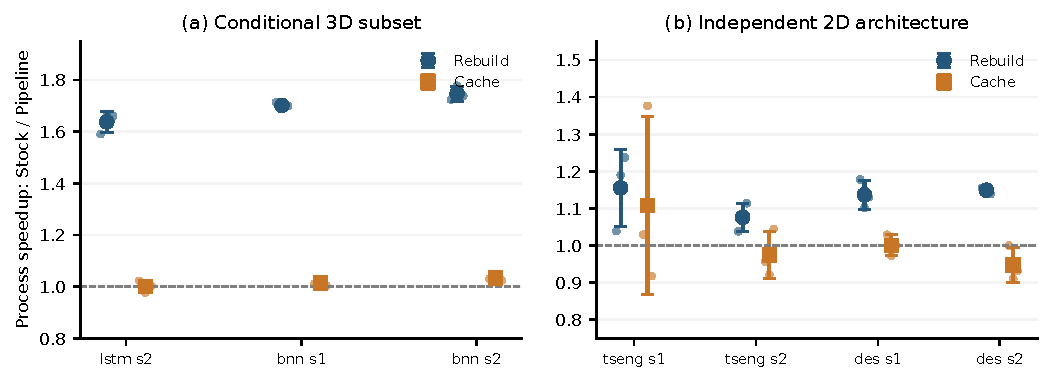
\includegraphics[width=.98\textwidth]{figures/expanded_endtoend.pdf}
\caption{Full-process paired speedups on two distinct cohorts. Markers and error bars show mean $\pm$ sample SD; small dots show all three pairs. The 3D subset was qualified in advance; k6 provides independent 2D architecture evidence. Shared-cache controls remove wire construction and support attribution, while retaining residual runtime variability.}
\label{fig:endtoend}
\end{figure*}

\subsection{Cache Reuse and Repeated Evaluation}
A cache hit bypasses the wire construction being optimized. GEMM's common-cache Stock-to-Pipeline result is \PrimaryCache\speedup, consistent with removal of the measured bottleneck. On the 3D conditional subset, equal-circuit cache aggregates are 1.012\speedup\ versus Stock and 0.996\speedup\ versus Group. These controls support construction as the main source of rebuild benefit; a speedup on a bypassed stage is not a requirement of the method.

Actual cache sequences on tseng and des evaluate three repeated batches per arm. Each batch first builds and writes its own equivalent table, then performs four requests using that table. For prefix length $K$, the measured batch time is
\begin{equation}
 B_a(K)=T_{a,\rm build}^{(1)}+\sum_{k=2}^{K}T_{a,\rm reuse}^{(k)}.
\end{equation}
Table~\ref{tab:cache} reports paired ratios of these sums. The $K=1,2,5$ prefixes share observations and are not independent experiments; the five requests use the same fixed design. These measured sequences demonstrate amortization without assuming that every placement change requires rebuilding a compatible table.

\begin{table}[t]
\centering\scriptsize
\caption{Measured cache-sequence speedups, control/Pipeline, mean $\pm$ sample SD over three batches. Prefixes are correlated.}
\label{tab:cache}
\setlength{\tabcolsep}{3pt}
\begin{tabular}{llrrr}
\toprule
Case & Control & $K=1$ & $K=2$ & $K=5$ \\
\midrule
\tableinput{tables/expanded_cache.tex}
\bottomrule
\end{tabular}
\end{table}

\subsection{Storage, Memory, and Representation Ablation}
Table~\ref{tab:memory} measures approximate stage RSS on instrumented eight-core runs after RR loading. Global scheduling increases workspace count from four to eight on the larger inputs, making additional concurrency a real memory tradeoff. For BNN-3D, observed growth is 162.0 MiB for Group, 231.7 MiB for Pipeline, and 241.1 MiB for Flat. Pipeline's sample-table bound is sixteen rather than Flat's forty. On BNN-2D, both global implementations have sixteen-sample bounds and nearly equal observed peaks.

\begin{table*}[t]
\centering\footnotesize
\caption{Stage memory diagnostics on host C, one instrumented observation per method (not performance repeats). RSS and label capacities are MiB. Peak is the maximum observed during construction, not an exact or guaranteed peak. Labels count wire-flood expanded/visited arrays only; table bounds exclude vector payloads, queues, allocator state, and common data.}
\label{tab:memory}
\setlength{\tabcolsep}{4pt}
\begin{tabular}{llrrrrrrr}
\toprule
Graph & Method & Entry RSS & Peak RSS & Growth & Label capacity & Workspaces & Sample bound & Group tables \\
\midrule
\tableinput{tables/expanded_memory.tex}
\bottomrule
\end{tabular}
\end{table*}

The sampler targets 2 ms but actual gaps can be much longer; observations can miss peaks. Earlier whole-process high-water marks were dominated by RR parsing and could not isolate construction growth. The newer measurements address that ambiguity, while remaining insufficient to claim a stable process-memory saving for Pipeline. The bounded representation limits a different object set and is not validated by subtracting these RSS samples.

Table~\ref{tab:ablation} retains the full storage/scheduling ablation. Compact cells and equivalent slice completion pass semantic checks, but the budgeted combination does not consistently improve process time over Pipeline. For eight-core GEMM, Bounded achieves $1.057\pm0.046$\speedup\ relative to Group, versus $1.093\pm0.003$\speedup\ for Pipeline; the paired Pipeline-time/Bounded-time ratio is $0.968\pm0.042$\speedup. The dependency and storage results remain useful methodological contributions, while Pipeline is retained as the main performance implementation.

\begin{table*}[t]
\centering\footnotesize
\caption{Representation/scheduling ablation: control Group time divided by candidate time, mean $\pm$ sample SD ($n=3$). All 120 formal native runs are legal and retain the reference wire-map bytes. Slice also includes a refactor; Compact versus Slice isolates representation in one executable, while Bounded changes scheduling and commit lifetimes together.}
\label{tab:ablation}
\setlength{\tabcolsep}{5pt}
\begin{tabular}{llrrrrr}
\toprule
Circuit & Cores & Mode & Slice & Compact & Pipeline & Bounded \\
\midrule
\tableinput{tables/ablation.tex}
\bottomrule
\end{tabular}
\end{table*}

\subsection{Alternative Models and Retained Failures}
The compatible compressed-map control is evaluated on tseng/des with its own quality gate rather than byte equality to the original map. Its des CPD changes by approximately $+3.95\%$, illustrating that alternative-model comparisons involve quality as well as runtime. It is not combined with the map-equivalent speedup aggregate. The locked compressed implementation's multilayer assertion is retained as an incompatibility, not counted as a victory for our method.

Earlier width-100 qualification attempted thirty runs across five variants and six large-design layouts: seventeen timed out, three stock runs crashed, five failed to converge, and five BNN-seed-2 runs were legal. The original formal matrix was not launched. Width-120 qualification retained three legal and three failed layouts. These results motivated separate all-graph construction and qualified full-flow studies, not selective removal of unfavorable performance observations. Fresh-layout small-design measurements and low-core regressions are likewise retained. The raw artifact distinguishes qualifications, diagnostics, capped routes, and complete formal runs.

\section{Implications for 3D CAD and Hardware Acceleration}
\subsection{A Faster Backend for Architecture and Placement Exploration}
LaZagna's customizable vertical connectivity and heterogeneous layer organization increase the number of meaningful architecture candidates~\cite{lazagna}. Each changed graph or cost model can require rebuilding lookahead. Our result reduces this repeated precomputation while preserving the baseline model, so architecture-quality comparisons can retain the same heuristic definition across CPU schedules. Cache reuse remains the preferred option when the graph and relevant cost state are compatible.

Escaping Flatland demonstrates the importance of accurate layer-dependent delay estimates and richer layer-assignment exploration~\cite{flatland}. Its four-dimensional placement-delay table and our six-index wire lookahead are related CAD components, not identical artifacts. Its improvements change placement guidance and quality; our experiments accelerate construction of an unchanged routing model. A future integration could combine improved placement with a faster routing-evaluation backend, and could apply the same independent-search decomposition to other precomputed delay tables after their own equivalence analysis. We have not measured that combined flow, and do not attribute its reported runtime overhead to our lookahead stage.

The practical opportunity is therefore a larger exploration budget: more architecture configurations, more placement candidates, or higher-fidelity models can be evaluated in a given time. A placement-only sweep may amortize construction through caching; a topology/cost sweep is more likely to repeatedly invoke it. Distinguishing these regimes makes the value proposition concrete without assuming universal reconstruction.

\subsection{An Execution Contract for Future Accelerators}
The present work resolves a dependency problem that additional hardware alone would not solve. If a host still dispatches one four-sample group and waits at its boundary, adding more engines cannot expose the forty independent searches already available in the graph. Our decomposition supplies a global task interface and a deterministic consumer boundary that can be retained when changing the execution backend.

A future accelerator can receive descriptors $(g,j,r_{g,j})$, read shared graph/cost data, maintain private search labels, and return layer-indexed $(d,q)$ records tagged with their original ordinal. An ordered collector then applies the same strict-delay rule and commits to the native layer-pair map. Pipeline token bounds provide backpressure at the result interface. The slice analysis identifies independent completion regions; compact cells reduce the structural cost of buffering their results. These are concrete design inputs for a replicated CPU/GPU/FPGA search engine, rather than a claim that CPU speedup transfers numerically to a device.

Several costs remain hardware-dependent: irregular RR memory access, priority queues, label initialization, graph transfer, queue/result buffering, and the precision/order needed for equivalent costs. Wire-label capacities and stage RSS quantify part of the replication cost, but not off-chip bandwidth or accelerator area. A hardware prototype must additionally demonstrate host/device transfer accounting, numerical equivalence, and a legal full-flow benefit. The CPU implementation provides a validated functional reference and task-level workload for that evaluation; no FPGA-board or GPU performance result is inferred here.

\subsection{Limits of the Current Evidence}
The method exposes available sample parallelism, not unlimited parallelism in every stage. Source/OPIN work, interpolation, ordered reduction, graph loading, and route checking can become residual bottlenecks. If construction occupies fraction $f$ of a process and accelerates by $a$, an unchanged-other-work model gives
\begin{equation}
 S_{\rm proc}=\frac{1}{1-f+f/a}.
\end{equation}
For optimized eight-core GEMM, the construction fraction is $(10.37\pm0.33)\%$; halving it would yield only about $1.055$\speedup\ in that idealized model. Further end-to-end gains require examining the remaining work, not continuing to extrapolate flood scaling.

Native 3D validation covers two layers and a limited set of vertical fabrics. More layers, different vertical resource densities, and heterogeneous sampling patterns require additional evaluation. Shared hosts and three runtime repeats limit inference about small differences; repeats do not replace independent circuits or layouts. The clma stage is short, and a preserved storage-preflight pause separates one BNN-2D stage pair. No rerun was substituted, but the interruption further limits interpretation of small stage differences. The substantive results are the large construction reductions, scaling beyond the group width, preserved native semantics, and measured benefits on qualified complete flows.

\section{Conclusion}
Multicore routing support does not by itself expose the parallelism available during lookahead construction. We decompose layer-aware native construction into independent floods, original-order cost reduction, and explicitly bounded execution/commit interfaces. Cross-group scheduling removes the four-sample group bottleneck and enables approximately twelvefold one-to-sixteen-core construction scaling on two large 3D graphs. At eight cores, GEMM process speedup is \PrimarySpeed\speedup; a qualified large 3D subset and independent 2D architectures corroborate full-flow benefit. Direct global-loop controls identify the source of the gain, while slice and storage studies expose further resource tradeoffs. The resulting execution contract provides an equivalent, measurable foundation for faster 3D architecture exploration and future hardware-parallel routing-cost computation.

\clearpage
\bibliographystyle{IEEEtran}
\bibliography{references}
\end{document}
